\documentclass[tikz,convert={size=640,density=300}]{standalone}
\usepackage{amsmath}
\usepackage{amssymb}
\usepackage{pgfplots}
\usepackage{pgfplotstable}
\usetikzlibrary{decorations.pathmorphing}
\usetikzlibrary{arrows}
\usetikzlibrary{calc}
\definecolor{pantone2727}{RGB}{48,127,226}
\definecolor{mymagenta}{RGB}{236,0,140}
\definecolor{myorange}{RGB}{209,115,0}
%\usetikzlibrary{...}% tikz package already loaded by 'tikz' option
\pgfplotsset{compat = newest}

\begin{document}

\def\xmin{-4}
\def\xmax{4}
\def\ymin{-4}
\def\ymax{4}
\def\xnomass{-0.5}
\def\xequil{-2}
\def\xcomp{0}
\def\xstretch{2}
\def\xone{-4}
\def\xtwo{4}
\def\yone{1}
\def\ytwo{1}
\def\thetaone{69.444}
\def\thetatwo{198.4349}

    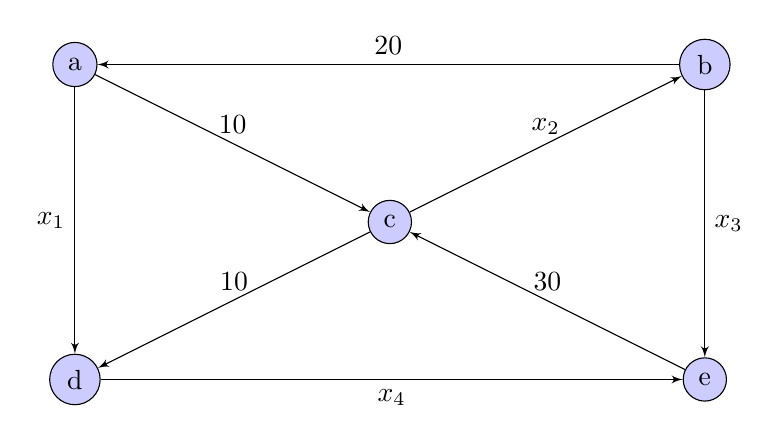
\begin{tikzpicture}
        \tikzset{vertex/.style = {shape=circle,draw,minimum size=1.5em,fill=blue!20}}
        \tikzset{edge/.style = {->,> = latex'}}        
        \node[vertex] (a) at (0,4) {a};
        \node[vertex] (b) at (8,4) {b};
        \node[vertex] (c) at (4,2) {c};
        \node[vertex] (d) at (0,0) {d};
        \node[vertex] (e) at (8,0) {e};

        \draw[edge] (a) -- (c) node[midway, above] {$10$};
        \draw[edge] (a) -- (d) node[midway, left] {$x_1$};
        \draw[edge] (b) -- (a) node[midway, above] {$20$};
        \draw[edge] (c) -- (b) node[midway, above] {$x_2$};
        \draw[edge] (b) -- (e) node[midway, right] {$x_3$};
        \draw[edge] (c) -- (d) node[midway, above] {$10$};
        \draw[edge] (e) -- (c) node[midway, above] {$30$}; 
        \draw[edge] (d) -- (e) node[midway, below] {$x_4$};
    \end{tikzpicture}
\end{document} 